\section{Contenuto e navigazione}

Come detto, l'assenza del \emph{breadcrumb} rischia di far confondere l'utente.
Tuttavia, in ogni pagina sono presenti altri strumenti di navigazione. Vediamoli più nel 
dettaglio.

\begin{figure}[hbt]
	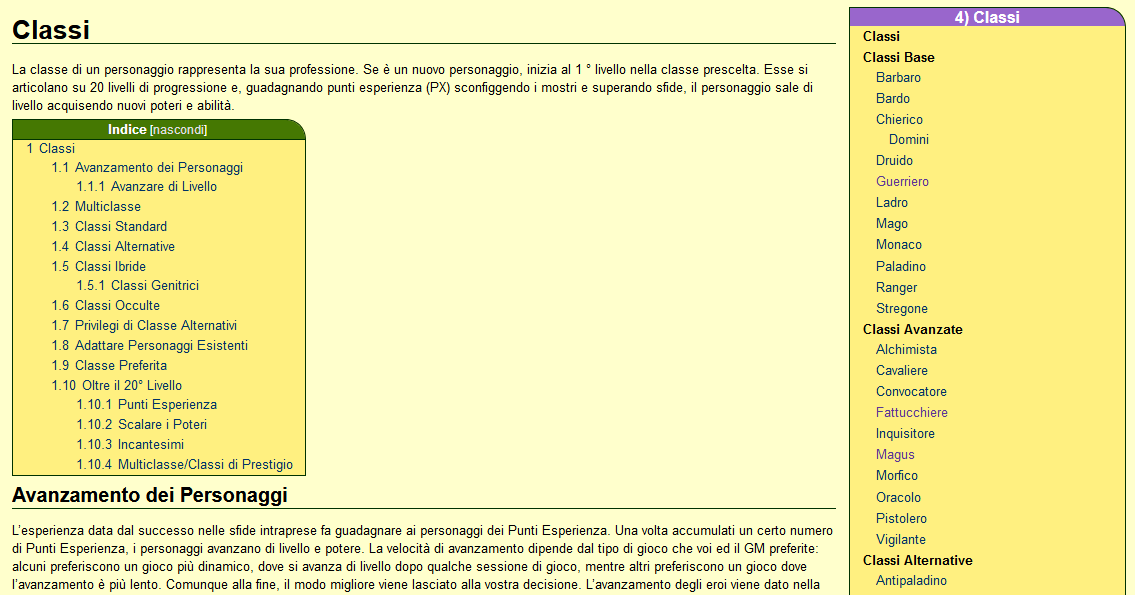
\includegraphics[width=\textwidth]{img/classi.png}
	\caption{\href{http://golarion.altervista.org/wiki/Classi}{Classi - Golarion Insider}}
\end{figure}

\begin{itemize}
	\item \textbf{Menù}: il menù a sinistra presente in ogni pagina, con i link principali (omesso nell'immagine). E' un menù a un solo livello, quindi non c'è nessun problema a tal riguardo;
	\item \textbf{Indice}: per le pagine più lunghe, come in questo caso, è presente un indice per 
	aiutare il visitatore a raggiungere, se necessario, il paragrafo specifico di suo interesse;
	\item \textbf{Menù di destra}: una raccolta di \emph{link} che porta alla pagina specifica della
	classe di interesse (in questo esempio. Il menù di destra varia in base alla pagina in cui si è).
\end{itemize}

\clearpage

\paragraph{Il paragrafo} I paragrafi, si presentano come nell'immagine sottostante. Come è possibile
vedere, il \emph{titolo} del paragrafo è ben distinto dal suo contenuto e le \emph{keywords} sono in genere link (in cui sono facilmente distinguibili i link non visitati da quelli visitati) che, in caso si voglia approfondire quell'argomento specifico, portano alla pagina di interesse.

\begin{figure}[hbt]
	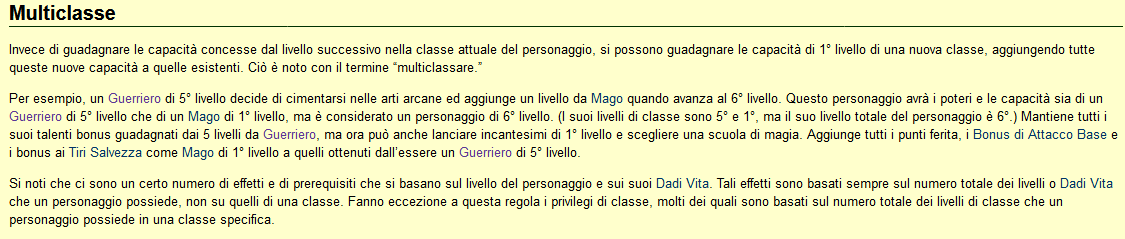
\includegraphics[width=\textwidth]{img/paragrafo.png}
	\caption{Un paragrafo, \href{http://golarion.altervista.org/wiki/Classi}{Classi - Golarion Insider}}
\end{figure}

